% II-4-6 Multithreaded Sorting Application - User and Operational Manual (LaTeX version of docs/Manual.md)
% Compile with XeLaTeX (twice, for the table of contents):
%   cd docs/manual
%   xelatex manual.tex
%   xelatex manual.tex
% Overleaf: Menu -> Compiler -> XeLaTeX. Upload docs/images/ next to this folder (paths are ../images/...).
\documentclass[11pt,a4paper]{article}

\usepackage{fontspec}
\usepackage{polyglossia}
\setdefaultlanguage{russian}   % Cyrillic hyphenation; Mongolian is not packaged in polyglossia
\setotherlanguage{english}

% Fonts with Mongolian Cyrillic (Ө, Ү). DejaVu is on Overleaf and most Linux systems,
% Times New Roman / Menlo are on macOS and Windows.
\IfFontExistsTF{DejaVu Serif}{
  \def\mainfam{DejaVu Serif}\def\sansfam{DejaVu Sans}\def\monofam{DejaVu Sans Mono}
}{
  \def\mainfam{Times New Roman}\def\sansfam{Arial}
  \IfFontExistsTF{Menlo}{\def\monofam{Menlo}}{\def\monofam{Courier New}}
}
\setmainfont{\mainfam}
\setsansfont{\sansfam}
\setmonofont{\monofam}[Scale=0.86]
\newfontfamily\cyrillicfont{\mainfam}
\newfontfamily\cyrillicfontsf{\sansfam}
\newfontfamily\cyrillicfonttt{\monofam}[Scale=0.86]

\usepackage[margin=2.2cm]{geometry}
\usepackage{graphicx}
\usepackage{xcolor}
\usepackage{booktabs}
\usepackage{longtable}
\usepackage{tabularx}
\usepackage{array}
\usepackage{enumitem}
\usepackage{fancyvrb}
\usepackage{fvextra}
\usepackage{caption}
\usepackage[hidelinks]{hyperref}

\definecolor{cleft}{HTML}{2F5BEA}
\definecolor{cright}{HTML}{D9860B}
\definecolor{cmerge}{HTML}{0E9A73}
\definecolor{ccmp}{HTML}{C2185B}
\definecolor{cmov}{HTML}{1B2433}
\definecolor{cused}{HTML}{C9CFD8}
\definecolor{codebg}{HTML}{F4F6F8}

\newcommand{\sw}[1]{\textcolor{#1}{\rule{0.9em}{0.9em}}}
\newcommand{\code}[1]{\texttt{#1}}
\DefineVerbatimEnvironment{cmd}{Verbatim}{fontsize=\small,frame=single,framesep=2mm,rulecolor=\color{cused},breaklines}
\setlist{itemsep=2pt,topsep=4pt}
% Mongolian captions (polyglossia has no Mongolian module, so override the Russian ones)
\gappto\captionsrussian{%
  \renewcommand{\contentsname}{Агуулга}%
  \renewcommand{\figurename}{Зураг}%
  \renewcommand{\tablename}{Хүснэгт}%
  \renewcommand{\partname}{Хэсэг}}
\emergencystretch=3em
\setlength{\parindent}{0pt}
\setlength{\parskip}{5pt}
\renewcommand{\arraystretch}{1.25}
\captionsetup{font=small}
\newcolumntype{Y}{>{\raggedright\arraybackslash}X}

\newcommand{\shot}[2]{%
  \begin{figure}[htbp]\centering
  \includegraphics[width=0.92\linewidth]{../images/#1}
  \caption{#2}
  \end{figure}}

\title{\textbf{II-4-6 Multithreaded Sorting Application}\\[4pt]\large Хэрэглэгчийн болон ашиглалтын гарын авлага}
\author{F.CSM302 Үйлдлийн систем, Бие даалт 1}
\date{2026}

\begin{document}
\begin{titlepage}
    \centering
    {\large \bfseries ШИНЖЛЭХ УХААН ТЕХНОЛОГИЙН ИХ СУРГУУЛЬ} \\[0.5cm]
    {\large МЭДЭЭЛЭЛ, ХОЛБООНЫ ТЕХНОЛОГИЙН СУРГУУЛЬ} \\[1.6cm]
    \IfFileExists{../../report/images/logo.png}{
\includegraphics[width=6cm]{../../report/images/logo.png}}{%
      \fbox{\parbox[c][3.5cm][c]{6cm}{\centering Лого:\\ \texttt{report/images/logo.png}}}} \\[1cm]
    {\Large \bfseries БИЕ ДААЛТ 1} \\[0.3cm]
    {\Large \bfseries ГАРЫН АВЛАГА} \\[0.3cm]
    {\normalsize (Хэрэглэгчийн ба operational заавар)} \\[0.5cm]
    {\large \bfseries Үйлдлийн систем (F.CSM302)} \\[1.8cm]
    \begin{tabular}{ll}
        \textbf{Сэдэв:} & Multithreaded Sorting Application, Sorting animation \\[0.3cm]
        \textbf{Хуваарилалтын код:} & II-4-6 \\[0.3cm]
        \textbf{Хичээл заасан багш:} & Г. Ганбат /F.CS10/ \\[0.3cm]
        \textbf{Гүйцэтгэсэн оюутнууд:} & Б. Отгондалай /B241940132/ \\
        & М. Мөнхгэрэлт /B232270012/ \\
        & А. Базарсад /B242270065/ \\
        & Б. Хаш-Эрдэнэ /B241930006/ \\
        & Э. Мичидмаа /B221960015/ \\
        & Ж. Суварнабазар /B251940118/ \\
    \end{tabular}
    \vfill
    {\large Улаанбаатар хот, 2026}
\end{titlepage}

Энэ гарын авлага хоёр хэсэгтэй:
\begin{itemize}
  \item \textbf{1. Хэрэглэгчийн заавар:} програмыг ашиглах хүнд зориулсан. Оролт оруулах, ажиллуулах,
        animation удирдах, өнгө ба төлөвийг унших, түгээмэл алдааг засахыг тайлбарлана.
  \item \textbf{2. Operational заавар:} төслийг шинэ машин дээр татаж, build хийж, тест ажиллуулж,
        үр дүнг шалгах хүнд (багш, шалгагч, багийн гишүүн) зориулсан.
\end{itemize}

\tableofcontents
\newpage

\section*{1. Хэрэглэгчийн заавар}\addcontentsline{toc}{part}{1. Хэрэглэгчийн заавар}

\section*{1.1 Програмын зорилго}\addcontentsline{toc}{section}{1.1 Програмын зорилго}
Програм бүхэл тоон жагсаалтыг \textbf{гурван бодит Java thread} ашиглан эрэмбэлнэ:
\begin{enumerate}
  \item \textbf{Parent thread} жагсаалтыг хоёр хэсэгт хуваана: зүүн хэсэг \code{[0, mid)}, баруун хэсэг \code{[mid, n)},
        энд $mid = \lceil n/2 \rceil$.
  \item Хоёр sorting thread (\textbf{Sorter-L}, \textbf{Sorter-R}) зэрэг эхэлж, тус бүр өөрийн хэсгийг сонгосон
        алгоритмаар эрэмбэлнэ. Thread бүр эхлэх, төгсөх индексээ параметрээр авна.
  \item Parent хоёр sorter-ийг \code{join()} хийсний дараа \textbf{Merger} thread-ийг эхлүүлнэ. Merger эрэмбэлэгдсэн
        хоёр хэсгийг \textbf{ижил хэмжээтэй хоёр дахь global массив} \code{result[]} руу нэгтгэнэ.
  \item Parent Merger-ийг \code{join()} хийгээд үр дүнг хэвлэнэ.
\end{enumerate}

Програмыг хоёр янзаар ашиглана:
\begin{itemize}
  \item \textbf{Командын мөр (CLI):} үр дүн, thread бүрийн статистик, хугацааг terminal дээр хэвлэнэ.
  \item \textbf{Web UI (Sorting animation):} хөтөч дээр массивыг багана хэлбэрээр харуулж, thread бүрийн алхмыг
        өнгөөр ялгана. Энэ animation нь зохиомол биш. Бодит thread-ийн хийсэн үйлдэл бүрийг event болгон
        бүртгэж, түүнийгээ харуулдаг.
\end{itemize}

\shot{01-start.png}{Web UI-ийн эхлэл}

\section*{1.2 Дэмжих орчин}\addcontentsline{toc}{section}{1.2 Дэмжих орчин}
\begin{tabularx}{\linewidth}{@{}lY@{}}
\toprule
Зүйл & Шаардлага \\
\midrule
Java & \textbf{JDK 17} буюу түүнээс дээш (\code{javac} хэрэгтэй, зөвхөн JRE хангалтгүй) \\
OS & macOS, Linux, Windows (Windows-ийн скриптийг бодит машин дээр туршаагүй, 2.9-р хэсгийг үзнэ үү) \\
Хөтөч & Web UI-д: Chrome, Edge, Firefox, Safari-ийн сүүлийн хувилбар \\
Гадны сан & Хэрэггүй (Maven, Gradle, JUnit, npm ашиглаагүй) \\
Сүлжээ & Хэрэггүй. Web сервер зөвхөн \code{127.0.0.1} дээр сонсоно \\
\bottomrule
\end{tabularx}

\section*{1.3 Суулгах, нээх}\addcontentsline{toc}{section}{1.3 Суулгах, нээх}
\textbf{macOS (Homebrew):}
\begin{cmd}
brew install --cask temurin@17
export JAVA_HOME=$(/usr/libexec/java_home -v 17)
javac -version
\end{cmd}

\textbf{Linux (Debian/Ubuntu):}
\begin{cmd}
sudo apt install openjdk-17-jdk
javac -version
\end{cmd}

\textbf{Windows:} \url{https://adoptium.net} хаягаас Temurin 17 (JDK)-г суулгаж, суулгах үед
“Set JAVA\_HOME” болон “Add to PATH” сонголтыг идэвхжүүлнэ. Дараа нь шинэ Command Prompt нээгээд
\code{javac -version} гэж шалгана.

\code{javac -version} нь \code{javac 17.x} (эсвэл түүнээс дээш) гэж харуулах ёстой. Дараа нь төслийн хавтсанд
\code{./build.sh} (Windows: \code{build.bat}) ажиллуулна. \code{Build OK (javac 17) -> out/} гэж гарвал бэлэн.

\section*{1.4 Оролт ба тохиргоо}\addcontentsline{toc}{section}{1.4 Оролт ба тохиргоо}
\subsection*{Оролтын дүрэм}
\begin{itemize}
  \item Зөвхөн \textbf{бүхэл тоо} (int муж: $-2\,147\,483\,648 \dots 2\,147\,483\,647$).
  \item Тусгаарлагч: таслал, цэг таслал, зай эсвэл шинэ мөр. Давхар таслалыг (\code{1,,2}) хоосон зай гэж үзээд алгасна.
  \item Сөрөг тоо (\code{-5}) болон \code{+} тэмдэг (\code{+3}) зөвшөөрнө. Давхардсан утга зөвшөөрнө.
  \item Файлд \code{\#} тэмдгээс хойших бичвэр тайлбар гэж тооцогдоно.
  \item \textbf{Сондгой n} зөвшөөрнө. Зүүн хэсэг $\lceil n/2\rceil$, баруун хэсэг $\lfloor n/2\rfloor$ элементтэй болно
        (жишээ нь n = 11 үед 6 ба 5).
\end{itemize}

\subsection*{CLI сонголтууд}
\begin{longtable}{@{}>{\ttfamily}p{0.32\linewidth}p{0.62\linewidth}@{}}
\toprule
\normalfont Сонголт & Утга \\
\midrule\endhead
--input "a,b,c" & Тоонуудыг шууд оруулах \\
a b c ... & Тоонуудыг аргумент болгон оруулах \\
--file PATH & Текст файлаас унших \\
--random N & N ширхэг санамсаргүй тоо үүсгэх \\
--seed S & Санамсаргүй тооны seed (ижил seed бол ижил жагсаалт) \\
--min A --max B & Санамсаргүй утгын муж (анхдагч 1..100) \\
--pattern P & \code{random}, \code{sorted}, \code{reversed}, \code{duplicates} \\
--algo NAME & Хоёр sorter-т ижил алгоритм (анхдагч \code{merge}) \\
--algo-left NAME & Sorter-L-ийн алгоритм \\
--algo-right NAME & Sorter-R-ийн алгоритм \\
--list-algos & Боломжит алгоритмын жагсаалт \\
--force & O(n²) алгоритмын n ≤ 20 000 хязгаарыг үл тоох \\
--full & n > 50 үед ч массивыг бүтнээр хэвлэх \\
--trace FILE & Бүх алхмыг JSON event trace болгон хадгалах (2.8) \\
--web [--port P] & Web UI-г эхлүүлэх (анхдагч порт 8080) \\
-h, --help & Тусламж \\
\bottomrule
\end{longtable}
Оролтын эх үүсвэрээс (\code{--input}, тоонууд, \code{--file}, \code{--random}) \textbf{яг нэгийг} өгнө.

\subsection*{Алгоритмууд}
\begin{tabularx}{\linewidth}{@{}>{\ttfamily}lYl@{}}
\toprule
\normalfont Нэр & Алгоритм & Хүндрэл \\
\midrule
insertion & Insertion sort & O(n²) \\
bubble & Bubble sort (эрт зогсолттой) & O(n²) \\
selection & Selection sort & O(n²) \\
merge & Merge sort (top-down, туслах буфертэй) & O(n log n) \\
quick & Quick sort (Hoare partition, дунд pivot) & O(n log n) дундаж \\
\bottomrule
\end{tabularx}

Зүүн ба баруун sorter-т \textbf{өөр өөр} алгоритм сонгож болно.

\subsection*{Web UI-ийн тохиргоо}
\begin{tabularx}{\linewidth}{@{}llY@{}}
\toprule
Хэсэг & Талбар & Тайлбар \\
\midrule
Өгөгдөл & Гараар / Санамсаргүй & Өгөгдлийн эх үүсвэр \\
 & Бүхэл тоонууд & Гараар оруулах жагсаалт. “Номын жишээ” товч номын жишээг бөглөнө \\
 & n, Seed, Min, Max, Хэлбэр & Санамсаргүй жагсаалт үүсгэх тохиргоо \\
Алгоритм & Sorter-L, Sorter-R & Хэсэг тус бүрийн алгоритм \\
Горим & Replay / Lockstep & Ажиллах горим (1.5) \\
\bottomrule
\end{tabularx}

\section*{1.5 Ажиллуулах, зогсоох, reset хийх}\addcontentsline{toc}{section}{1.5 Ажиллуулах, зогсоох, reset хийх}
\subsection*{Командын мөр}
\begin{cmd}
./run.sh --input "7,12,19,3,18,4,2,6,15,8"
\end{cmd}
Гаралт:
\begin{cmd}
Оролт: гараас оруулсан
Эх жагсаалт (n=10): [7, 12, 19, 3, 18, 4, 2, 6, 15, 8]
Хуваалт: зүүн [0,5) хэмжээ 5, баруун [5,10) хэмжээ 5
[Sorter-L] tid=18 муж=[0,5) merge: compare=7 swap=0 write=12, 1.347-1.391 ms
[Sorter-R] tid=19 муж=[5,10) merge: compare=5 swap=0 write=12, 1.538-1.549 ms
[Merger] tid=20 нэгтгэл list[0,5) + list[5,10) -> result[0,10): compare=8 write=10, 2.483-2.514 ms
Parent thread бүх thread-ийг join хийлээ.
Эрэмбэлсэн үр дүн: [2, 3, 4, 6, 7, 8, 12, 15, 18, 19]
Шалгалт (Arrays.sort-той харьцуулав): ЗӨВ
Хугацаа: эрэмбэлэх үе 1.574 ms, нийт 2.550 ms
\end{cmd}

\begin{itemize}
  \item \code{tid}: Java thread-ийн дугаар. Гурван thread гурван өөр дугаартай байгаа нь тэд тусдаа thread гэдгийг харуулна.
  \item \code{муж}: thread-д параметрээр дамжуулсан индексийн муж.
  \item \code{compare / swap / write}: тухайн thread-ийн хийсэн үйлдлийн тоо.
  \item \code{1.347-1.391 ms}: run эхэлснээс хойш тухайн thread эхэлсэн ба дууссан хугацаа.
  \item \code{Шалгалт}: үр дүнг \code{java.util.Arrays.sort}-той харьцуулсан дүн.
\end{itemize}
CLI ажиллаад дуусахдаа өөрөө зогсоно. Exit code: \code{0} амжилттай, \code{1} үр дүн буруу (хэвийн үед гарахгүй),
\code{2} оролтын алдаа.

\subsection*{Web UI (Sorting animation)}
\begin{cmd}
./run.sh --web
\end{cmd}
Terminal дээр \code{Sorting animation сервер ажиллаж байна: http://localhost:8080/} гэж гарна. Хөтөч дээр
\url{http://localhost:8080} хаягийг нээнэ.
\begin{itemize}
  \item Өөр порт: \code{./run.sh --web --port 8100}.
  \item \textbf{Зогсоох:} серверийг ажиллуулсан terminal дээр \code{Ctrl+C}.
  \item Хөтчийн цонхыг хаахад ажиллаж буй Lockstep session автоматаар цуцлагдана.
\end{itemize}

\subsection*{Хоёр горим}
\begin{tabularx}{\linewidth}{@{}>{\raggedright}p{0.17\linewidth}YY@{}}
\toprule
 & \textbf{Replay} & \textbf{Lockstep} \\
\midrule
Юу болдог & Java дээр 3 бодит thread бүрэн ажиллаж дуусна. Бүртгэсэн event-үүдийг хөтөч дээр тоглуулна
  & Java thread-үүд \textbf{амьд} хэвээр байна. Үйлдэл бүрийн өмнө \code{Semaphore}-ийн permit хүлээж,
    бодитоор \code{WAITING} төлөвт зогсоно \\
“Алхам ▸” & Дараагийн бүртгэсэн event-ийг харуулна & Серверт нэг permit өгнө, нэг thread яг \textbf{нэг} үйлдэл хийнэ \\
Хойш алхах & Болно (◂ Алхам, Байрлал гулсуур) & \textbf{Болохгүй}, бодит thread-ийг буцааж болдоггүй \\
Хугацаа & Бодит хурдыг харуулна & Таны товч дарах хоорондын хугацааг багтаана \\
Хамгийн их n & 300 & 100 \\
\bottomrule
\end{tabularx}

Хурд хэмжих бол \textbf{Replay}, thread-ийн төлөвийг (\code{WAITING}, \code{RUNNABLE}, \code{TERMINATED}) бодитоор
харах бол \textbf{Lockstep} горимыг ашиглана.

\subsection*{Товч ба удирдлага}
\begin{tabularx}{\linewidth}{@{}lYl@{}}
\toprule
Удирдлага & Үйлдэл & Гарын товч \\
\midrule
\textbf{Ажиллуулах} & Java дээр шинэ run эхлүүлнэ & \\
\textbf{Тоглуулах / Түр зогсоох} & Тасралтгүй тоглуулах эсвэл зогсоох & Space \\
\textbf{Алхам ▸} & Нэг алхам урагшлах & → \\
\textbf{◂ Алхам} & Нэг алхам хойшлох (зөвхөн Replay) & ← \\
\textbf{Эхнээс нь} & Replay: эхлэл рүү буцна. Lockstep: шинэ session эхлүүлнэ & \\
\textbf{Хурд} & 1-ээс 5000 алхам/сек (логарифм шкал) & \\
\textbf{Байрлал} & Гулсуураар дурын event рүү үсрэх (зөвхөн Replay) & \\
\bottomrule
\end{tabularx}

Горимыг солиход өмнөх дүрслэл цэвэрлэгдэж, ажиллаж байсан Lockstep session цуцлагдана. Дараа нь
“Ажиллуулах”-ыг дахин дарна.

\section*{1.6 Дүрслэлийн тэмдэг, өнгө, төлөв}\addcontentsline{toc}{section}{1.6 Дүрслэлийн тэмдэг, өнгө, төлөв}
\subsection*{Баганы өнгө}
\begin{tabularx}{\linewidth}{@{}lY@{}}
\toprule
Өнгө & Утга \\
\midrule
\sw{cleft}\ Цэнхэр & Sorter-L-ийн хэсэг \code{[0, mid)} \\
\sw{cright}\ Улбар шар & Sorter-R-ийн хэсэг \code{[mid, n)} \\
\sw{cmerge}\ Ногоон & Merger-ийн \code{result[]}-д бичсэн утга \\
\sw{ccmp}\ Ягаан улаан & Яг одоо харьцуулж буй элементүүд \\
\sw{cmov}\ Хар & Яг одоо сольсон эсвэл бичсэн элемент \\
\sw{cused}\ Саарал & Merger аль хэдийн авсан элемент \\
\textcolor{cmov}{\rule{1.5pt}{0.9em}}\ Босоо зураас & Хуваалтын цэг \code{mid} \\
\bottomrule
\end{tabularx}

Merger ажиллах үед \code{list[]} дээр \code{i} (зүүн хэсгийн заагч), \code{j} (баруун хэсгийн заагч) тэмдэг гарна.

\subsection*{Дэлгэцийн хэсгүүд}
\begin{enumerate}
  \item \textbf{Дээд самбар:} өгөгдөл, алгоритм, горим, удирдлагын товчнууд, хурд ба байрлалын гулсуур.
  \item \textbf{Эх массив \code{list[]}:} хоёр sorter өөрийн хэсгийг энд эрэмбэлнэ.
  \item \textbf{Хоёр дахь global массив \code{result[]}:} Merger энд нэгтгэнэ.
  \item \textbf{Thread-ийн хугацааны шугам:} thread бүр хэзээ ажилласныг бодит \code{System.nanoTime} хугацаагаар
        харуулна. Parent-ийн мөрөнд \code{start()} / \code{join()} агшнууд босоо зураасаар гарна.
  \item \textbf{Thread-ийн картууд:} нэр, \code{tid}, төлөв, муж, үйлдлийн тоо.
  \item \textbf{Сүүлийн event-үүд:} сүүлд болсон алхмууд, thread бүр өөрийн өнгөтэй.
  \item \textbf{Үр дүн:} оролт, эрэмбэлсэн үр дүн, шалгалт, хугацаа (trace-тэй ба trace-гүй), event-ийн тоо.
\end{enumerate}

\subsection*{Thread-ийн төлөв}
\begin{tabularx}{\linewidth}{@{}lY@{}}
\toprule
Төлөв (карт) & Утга \\
\midrule
Үүсээгүй & Thread объект хараахан үүсээгүй \\
start() дуудагдсан & Parent \code{start()} дуудсан, thread эхэлж амжаагүй \\
Ажиллаж байна & Thread өөрийн ажлыг хийж байна \\
join() дээр хүлээж байна & (Parent) хүүхэд thread-ээ дуусахыг хүлээж байна \\
Дууссан & Thread-ийн \code{run()} дууссан \\
\bottomrule
\end{tabularx}

\textbf{Lockstep} горимд карт дээр нэмэлт \textbf{Java төлөв} (\code{Thread.getState()}) гарна:

\begin{tabularx}{\linewidth}{@{}>{\ttfamily}lY@{}}
\toprule
\normalfont Java төлөв & Утга \\
\midrule
NEW & \code{new Thread()} хийгдсэн, \code{start()} дуудаагүй \\
RUNNABLE & Ажиллаж байна \\
WAITING & Sorter/Merger: Semaphore permit хүлээж байна. Parent: \code{join()} дээр хүлээж байна \\
TERMINATED & Дууссан \\
\bottomrule
\end{tabularx}

\section*{1.7 Жишээ}\addcontentsline{toc}{section}{1.7 Жишээ}
\subsection*{Жишээ 1. Номын жишээ (Web UI, Replay)}
\begin{enumerate}
  \item \code{./run.sh --web} ажиллуулж, \url{http://localhost:8080} хаягийг нээнэ.
  \item “Номын жишээ” товчийг дарна: \code{7, 12, 19, 3, 18, 4, 2, 6, 15, 8}.
  \item Sorter-L-д \code{insertion}, Sorter-R-д \code{merge} сонгоно.
  \item \textbf{Ажиллуулах}, дараа нь \textbf{Алхам ▸}-ийг хэд дарж, Sorter-L өөрийн хэсгийг insertion sort-оор
        эрэмбэлж буйг харна (Зураг~\ref{fig:sorting}).
  \item \textbf{Байрлал} гулсуурыг төгсгөл рүү чирвэл Merger \code{result[]}-ийг ногооноор бөглөж буй нь харагдана
        (Зураг~\ref{fig:merge}).
  \item Төгсгөлд нь \code{result[] = 2 3 4 6 7 8 12 15 18 19}, Шалгалт: “Эрэмбэлэгдсэн, зөв” (Зураг~\ref{fig:done}).
\end{enumerate}

\begin{figure}[htbp]\centering
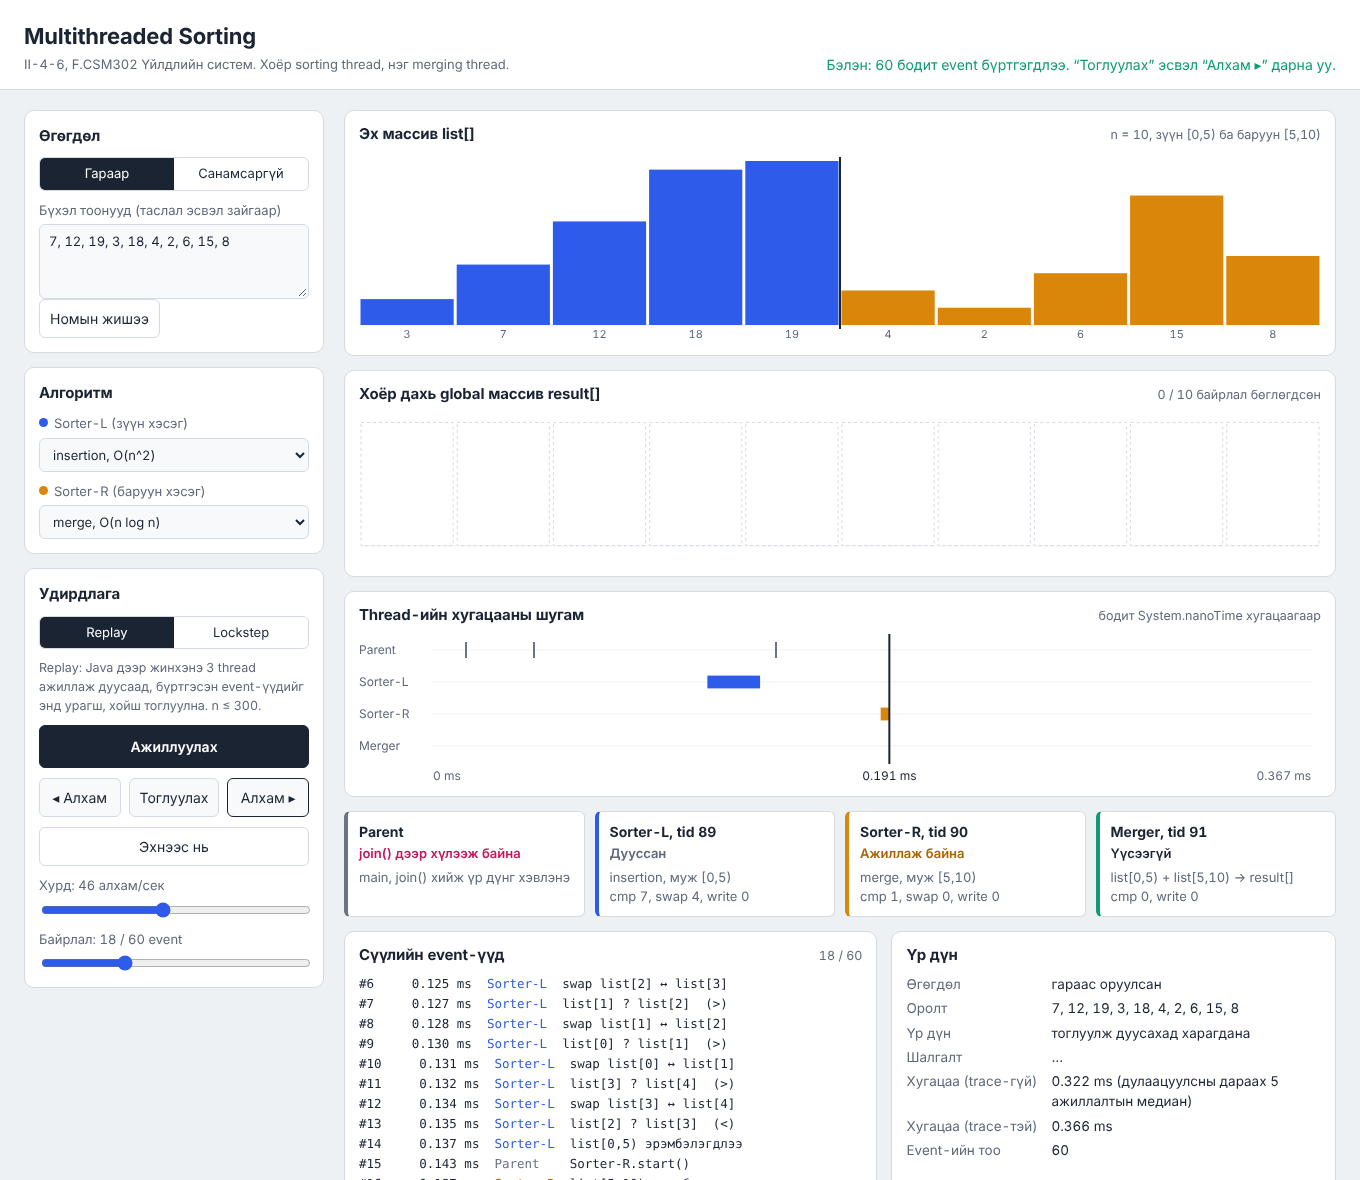
\includegraphics[width=0.92\linewidth]{../images/02-replay-sorting.png}
\caption{Sorter-L ажиллаж байна}\label{fig:sorting}
\end{figure}
\begin{figure}[htbp]\centering
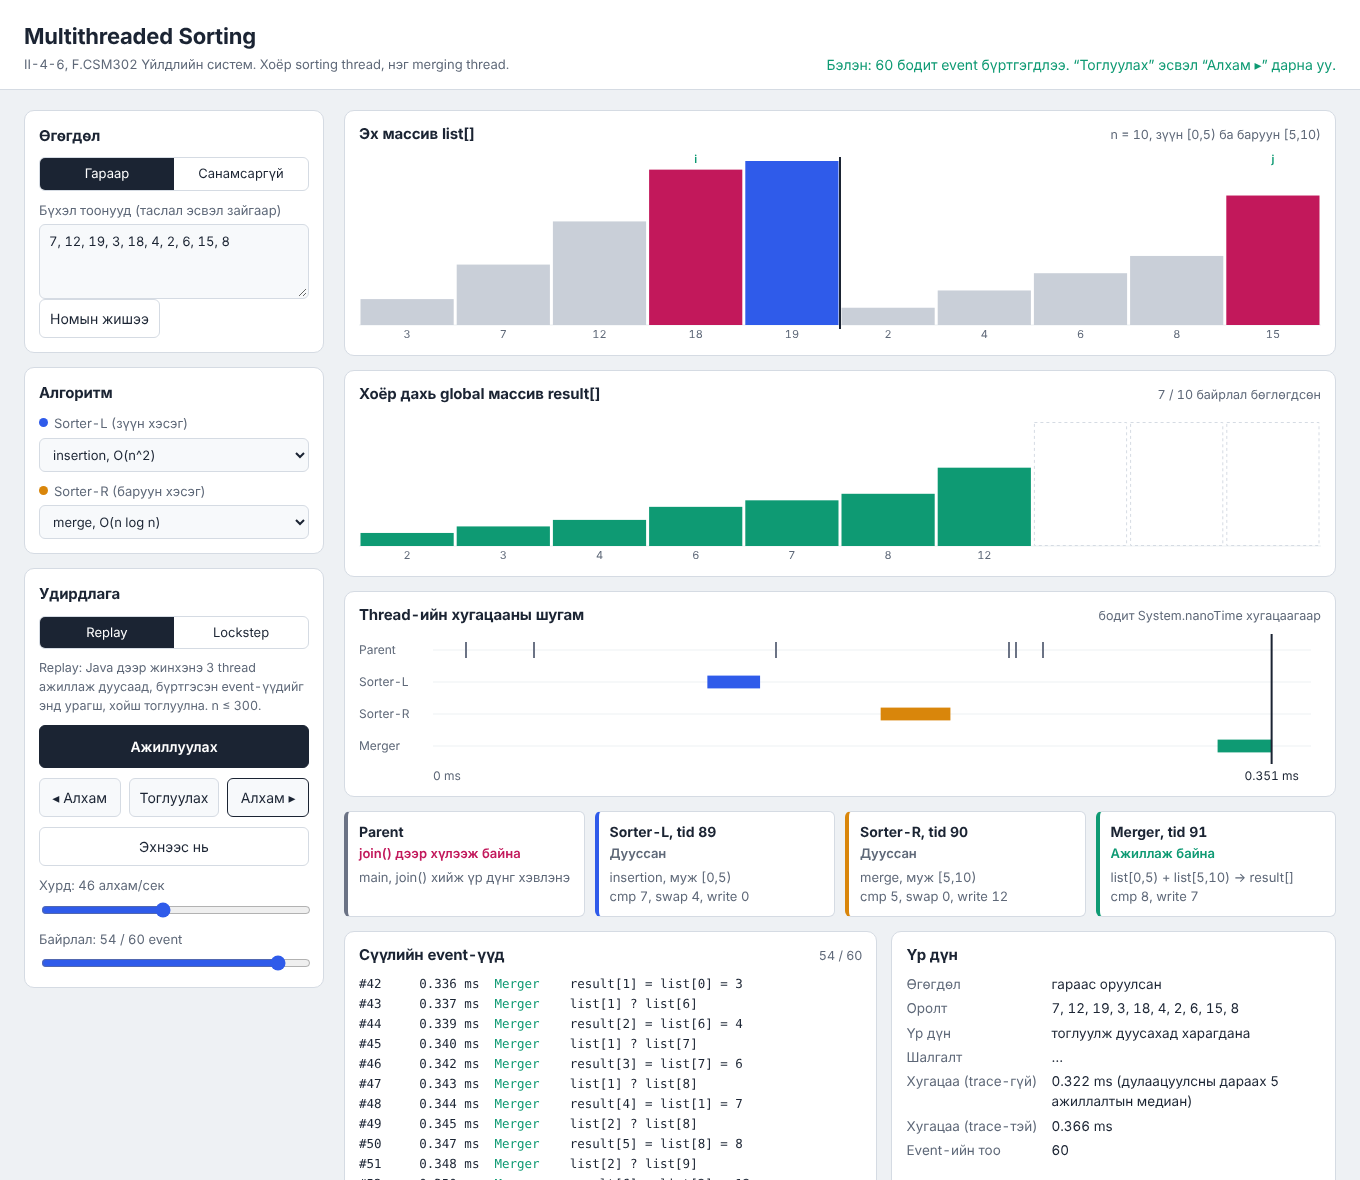
\includegraphics[width=0.92\linewidth]{../images/03-replay-merge.png}
\caption{Merger нэгтгэж байна}\label{fig:merge}
\end{figure}
\begin{figure}[htbp]\centering
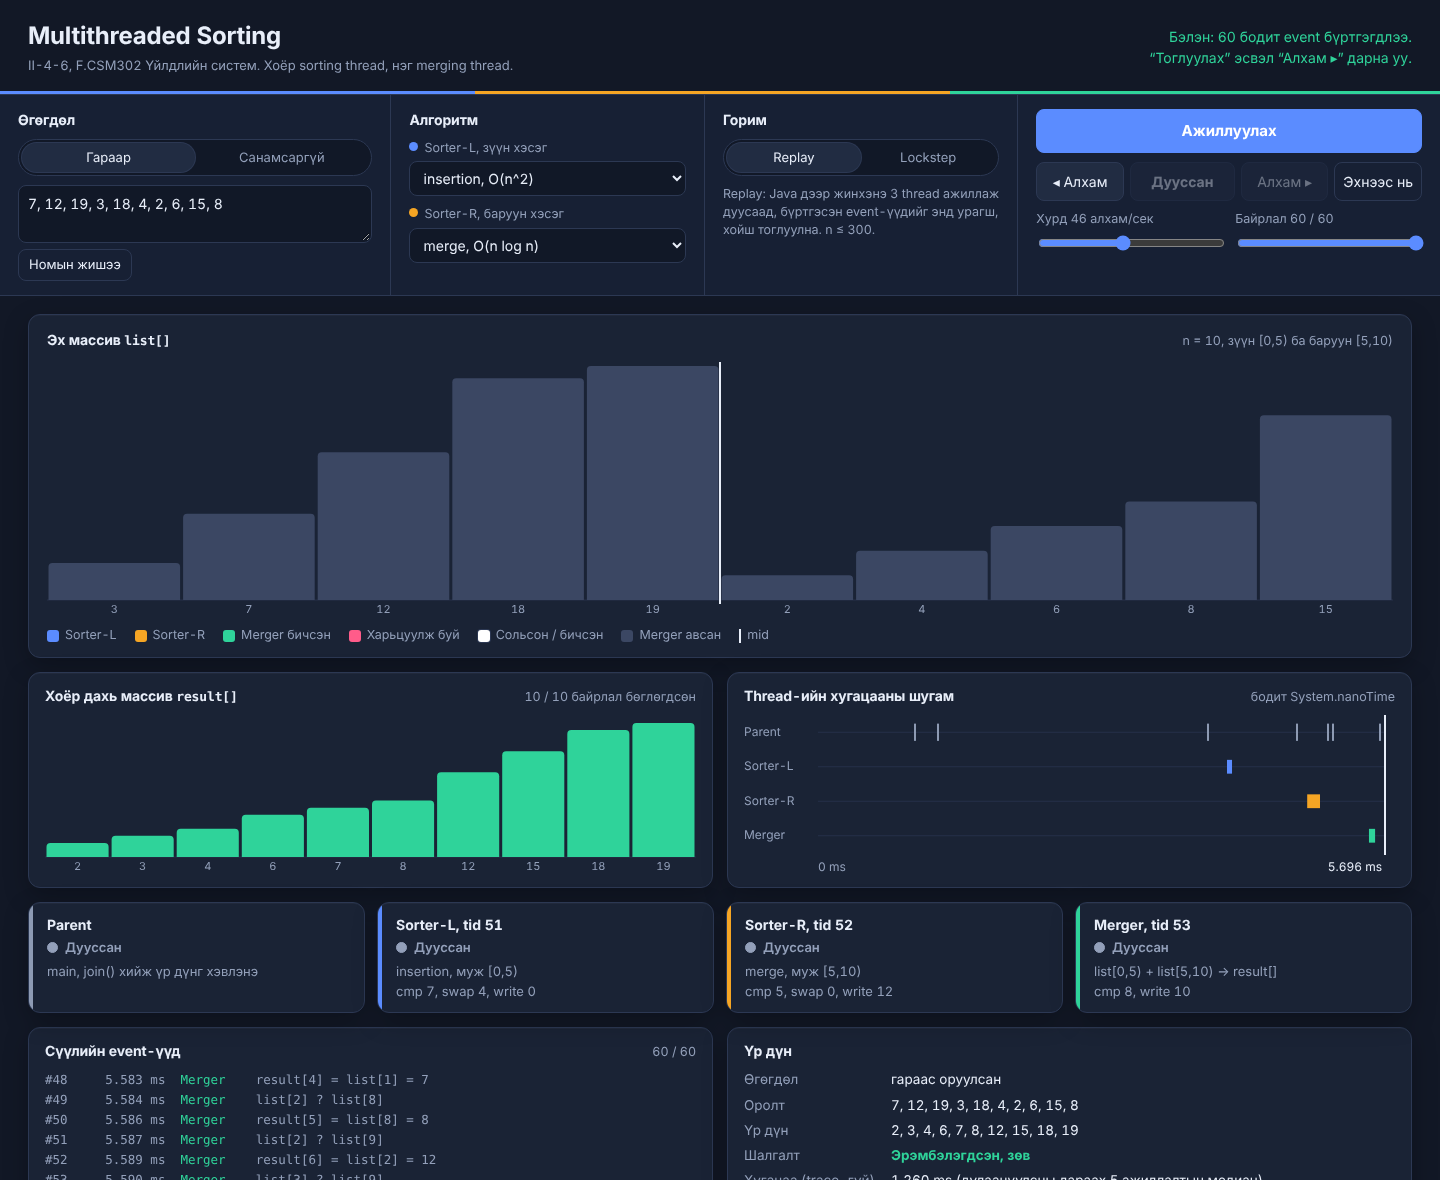
\includegraphics[width=0.92\linewidth]{../images/04-replay-done.png}
\caption{Дууссан төлөв}\label{fig:done}
\end{figure}

\subsection*{Жишээ 2. Сондгой n ба өөр алгоритм (CLI)}
\begin{cmd}
./run.sh --file examples/odd-11.txt --algo-left bubble --algo-right quick
\end{cmd}
Хүлээгдэх үр дүн:
\begin{cmd}
Тэмдэглэл: n = 11 сондгой тул зүүн хэсэг 6, баруун хэсэг 5 элементтэй (⌈n/2⌉ / ⌊n/2⌋).
Хуваалт: зүүн [0,6) хэмжээ 6, баруун [6,11) хэмжээ 5
Эрэмбэлсэн үр дүн: [1, 2, 3, 4, 5, 6, 7, 8, 9, 10, 11]
Шалгалт (Arrays.sort-той харьцуулав): ЗӨВ
\end{cmd}

\subsection*{Жишээ 3. Санамсаргүй 60 тоо (Web UI)}
“Санамсаргүй” сонгож n = 60, Seed = 42, Sorter-L = \code{bubble}, Sorter-R = \code{quick} гэж тохируулаад
Ажиллуулна. Хоёр sorter-ийн хугацааны шугам давхцаж байгаа нь тэд \textbf{зэрэг} ажилласныг харуулна.

\shot{05-random-60.png}{Санамсаргүй 60 тоо, bubble + quick}

\subsection*{Жишээ 4. Lockstep горим}
\begin{enumerate}
  \item Дээд самбарын “Горим” хэсэгт \textbf{Lockstep} сонгоно.
  \item \textbf{Ажиллуулах} дарна. Карт дээр Sorter-L ба Sorter-R: \code{Java: WAITING, Semaphore permit хүлээж байна},
        Parent: \code{Java: WAITING, join() дээр} гэж гарна.
  \item \textbf{Алхам ▸} бүрд нэг thread нэг үйлдэл хийнэ. Fair (FIFO) semaphore ашигладаг тул хоёр sorter ээлжилнэ
        (L, R, L, R \dots\ эсвэл R, L, R, L \dots).
  \item \textbf{Тоглуулах} дарвал хурдны тохиргооны дагуу permit-ийг тасралтгүй өгнө. Төгсгөлд бүх thread
        \code{TERMINATED} болно.
\end{enumerate}

\shot{06-lockstep.png}{Lockstep горим: бодит thread-үүд Semaphore дээр WAITING}

\section*{1.8 Түгээмэл алдаа ба шийдэл}\addcontentsline{toc}{section}{1.8 Түгээмэл алдаа ба шийдэл}
\begin{longtable}{@{}>{\raggedright}p{0.40\linewidth}>{\raggedright}p{0.22\linewidth}>{\raggedright\arraybackslash}p{0.32\linewidth}@{}}
\toprule
Алдааны мессеж & Шалтгаан & Шийдэл \\
\midrule\endhead
\code{javac олдсонгүй} & JDK суугаагүй & 1.3-р хэсгийг үзнэ үү \\
\code{JDK 17+ хэрэгтэй, гэтэл одоогийн javac хувилбар: 11} & Хуучин Java PATH-д байна & macOS: \code{export JAVA\_HOME=}\newline\code{\$(/usr/libexec/java\_home -v 17)} \\
\code{out/ олдсонгүй. Эхлээд ./build.sh ажиллуулна уу.} & Build хийгээгүй & \code{./build.sh} \\
\code{Оролтын өгөгдөл өгөөгүй байна} & Оролтын эх үүсвэр алга & \code{--input}, \code{--file} эсвэл \code{--random} \\
\code{Оролт хоосон байна} & Хоосон жагсаалт & Дор хаяж нэг тоо \\
\code{3-р утга 'abc' нь бүхэл тоо биш.} & Тоо биш утга & Зөвхөн бүхэл тоо \\
\code{2-р утга '2.5' нь бутархай тоо.} & Бутархай тоо & Бүхэл тоо оруулна \\
\code{2-р утга '3000000000' нь int мужаас хэтэрсэн.} & Хэт том/бага тоо & int мужид оруулна \\
\code{insertion нь O(n\textasciicircum 2) алгоритм тул n ≤ 20000 ...} & O(n²)-д n хэт их & \code{merge}/\code{quick}, n багасгах, эсвэл \code{--force} \\
\code{'foo' гэсэн алгоритм байхгүй} & Алгоритмын нэр буруу & \code{--list-algos} \\
\code{Файл олдсонгүй: ...} & Файлын зам буруу & Төслийн хавтсаас эхлэх зам \\
\code{min (9) нь max (1)-аас их байж болохгүй.} & Муж буруу & min ≤ max \\
\code{8080 порт аль хэдийн ашиглагдаж байна} & Портыг өөр програм эзэлсэн & \code{--port 8100} эсвэл өмнөх серверийг \code{Ctrl+C} \\
Хөтөч: \code{Сервертэй холбогдож чадсангүй} & Сервер зогссон & \code{./run.sh --web} дахин \\
\code{Lockstep session олдсонгүй} & 10 минут хөдөлгөөнгүй эсвэл сервер дахин асаасан & “Ажиллуулах” дахин \\
zsh: \code{command not found: \#} & Командыг тайлбартай нь хуулсан & Зөвхөн командын мөрийг хуулна \\
\bottomrule
\end{longtable}

\shot{07-error.png}{Буруу оролтын алдааны мессеж}

\section*{1.9 Хязгаарлалт}\addcontentsline{toc}{section}{1.9 Хязгаарлалт}
\begin{tabularx}{\linewidth}{@{}>{\raggedright}p{0.36\linewidth}>{\raggedright}p{0.26\linewidth}Y@{}}
\toprule
Зүйл & Хязгаар & Шалтгаан \\
\midrule
Утга & int муж & Java \code{int} \\
O(n²) алгоритм (insertion, bubble, selection) & n ≤ 20 000 (\code{--force}-оор давж болно) & Удаан ажиллахаас сэргийлнэ \\
O(n log n) алгоритм (merge, quick) & n ≤ 1 000 000 & Санах ой, хугацаа \\
\code{--trace}, O(n²) алгоритмтай & n ≤ 1 000 & Алхам бүр нэг event тул файл хэт томорно \\
\code{--trace}, merge/quick & n ≤ 10 000 & Мөн адил \\
Web UI, Replay & n ≤ 300 & Animation уншигдахуйц байх \\
Web UI, Lockstep & n ≤ 100 & Алхам бүр серверт хүсэлт явуулна \\
Зэрэг Lockstep session & 4 & 10 минут хөдөлгөөнгүй session автоматаар цуцлагдана \\
\bottomrule
\end{tabularx}

\clearpage
\section*{2. Operational заавар}\addcontentsline{toc}{part}{2. Operational заавар}

\section*{2.1 Repository clone хийх}\addcontentsline{toc}{section}{2.1 Repository clone хийх}
\begin{cmd}
git clone https://github.com/Munkhgerelt/F.CSM302-TeamProject-2-4-6.git
cd F.CSM302-TeamProject-2-4-6
\end{cmd}

\section*{2.2 OS, compiler/runtime, хувилбар}\addcontentsline{toc}{section}{2.2 OS, compiler/runtime, хувилбар}
\begin{tabularx}{\linewidth}{@{}>{\raggedright}p{0.24\linewidth}>{\raggedright}p{0.27\linewidth}>{\raggedright}p{0.25\linewidth}Y@{}}
\toprule
Орчин & OS & JDK & Үр дүн \\
\midrule
Багийн гишүүний компьютер & macOS 27 (Apple Silicon, aarch64), 10 цөм & Eclipse Temurin 17.0.21+9 & Build OK, тест 100/100 \\
Хөгжүүлэлтийн Linux контейнер & Ubuntu 24.04 (amd64), 2 цөм & OpenJDK 21 (\code{--release 17}) & Build OK, тест 100/100 \\
Windows & Туршаагүй & & 2.9 \\
\bottomrule
\end{tabularx}

\code{build.sh} нь \code{javac --release 17} ашигладаг. Тиймээс JDK 21 дээр build хийсэн ч Java 17-д ажиллах код гарна.

\section*{2.3 Dependency суулгах}\addcontentsline{toc}{section}{2.3 Dependency суулгах}
Програм нь гадны ямар ч сан ашигладаггүй тул зөвхөн JDK 17 буюу түүнээс дээш хувилбар хэрэгтэй (1.3-р хэсэг).
Maven, Gradle, npm, JUnit суулгах шаардлагагүй. Web UI нь JDK-д багтсан \code{com.sun.net.httpserver}-ийг ашигладаг
тул тусдаа web сервер ч хэрэггүй.

\section*{2.4 Build ба Run}\addcontentsline{toc}{section}{2.4 Build ба Run}
\begin{tabularx}{\linewidth}{@{}lYY@{}}
\toprule
Үйлдэл & macOS / Linux & Windows \\
\midrule
Build & \code{./build.sh} & \code{build.bat} \\
CLI & \code{./run.sh --file examples/book-example.txt} & \code{run.bat --file examples\textbackslash book-example.txt} \\
Web UI & \code{./run.sh --web} & \code{run.bat --web} \\
Тест & \code{./test.sh} & \code{test.bat} \\
\bottomrule
\end{tabularx}

Скрипт ажиллуулах эрхгүй бол \code{chmod +x build.sh run.sh test.sh} хийнэ. \code{build.sh} нь:
\begin{enumerate}
  \item \code{javac}-ийн хувилбарыг шалгана (17-оос доош бол алдаа өгч, зааварчилгаа хэвлэнэ);
  \item \code{src/main/java} доторх бүх \code{.java} файлыг \code{out/} руу хөрвүүлнэ;
  \item \code{src/main/resources/web} (HTML/CSS/JS)-ийг \code{out/} руу хуулна.
\end{enumerate}
\code{out/}, \code{out-test/} хавтас, \code{.class} файлууд нь \code{.gitignore}-д орсон тул commit хийгдэхгүй.

\section*{2.5 Үндсэн тестийн өгөгдөл}\addcontentsline{toc}{section}{2.5 Үндсэн тестийн өгөгдөл}
\begin{tabularx}{\linewidth}{@{}>{\ttfamily}l>{\raggedright}p{0.27\linewidth}Y@{}}
\toprule
\normalfont Файл (\code{examples/}) & Агуулга & Хүлээгдэх үр дүн \\
\midrule
book-example.txt & Номын жишээ, n = 10 & \code{2 3 4 6 7 8 12 15 18 19} \\
odd-11.txt & Сондгой n = 11 & Хуваалт 6 / 5, \code{1 2 \dots\ 11} \\
duplicates.txt & Давхардсан утга, n = 12 & \code{1 1 1 2 2 3 3 3 3 5 5 5} \\
reversed.txt & Урвуу эрэмбэ, n = 10 & \code{1 2 \dots\ 10} \\
int-limits.txt & Сөрөг тоо, INT\_MIN, INT\_MAX & \code{-2147483648 -100 -1 0 0 7 100 2147483647} \\
single.txt & Ганц элемент & \code{42}, баруун хэсэг хоосон \\
invalid-letters.txt & \code{abc} агуулсан & Алдаа, exit code 2 \\
invalid-overflow.txt & \code{3000000000} & Алдаа, exit code 2 \\
empty.txt & Зөвхөн тайлбар & Алдаа, exit code 2 \\
\bottomrule
\end{tabularx}

Санамсаргүй өгөгдлийг \code{--random N --seed S --pattern P} сонголтоор давтагдахуйц үүсгэнэ.

\section*{2.6 Автомат тест ба хүлээгдсэн үр дүн}\addcontentsline{toc}{section}{2.6 Автомат тест ба хүлээгдсэн үр дүн}
\begin{cmd}
./test.sh
\end{cmd}
Скрипт build хийж, \code{tests/TestRunner.java}-г хөрвүүлж ажиллуулна (JUnit-гүй, цэвэр Java 17, ойролцоогоор
5--10 секунд). Төгсгөлд нь:
\begin{cmd}
Нийт: 100, амжилттай: 100, алдаатай: 0
Хүснэгт: tests/results/test-results.md
\end{cmd}
\code{tests/results/test-results.md} файлд тест бүрийн \textbf{оролт, хүлээгдсэн утга, бодит утга, үр дүн}
хүснэгтээр бичигдэнэ. Хүлээгдсэн утгыг тестийн кодонд урьдчилан бичсэн бөгөөд бодит утга нь програмыг
ажиллуулж гарсан үр дүн юм. Бүх тест амжилттай бол exit code 0, үгүй бол 1.

\begin{tabularx}{\linewidth}{@{}lrY@{}}
\toprule
Ангилал & Тоо & Шалгах зүйл \\
\midrule
Номын жишээ & 26 & 5 × 5 = 25 алгоритмын хослол, хуваалт ба хоёр хэсэг \\
Захын тохиолдол & 17 & n = 1, 2, 3, бүгд ижил, сөрөг, INT\_MIN/MAX, эрэмбэтэй/урвуу, ⌈n/2⌉/⌊n/2⌋ \\
Буруу оролт & 18 & Хоосон, тоо биш, бутархай, int-ээс гадуур, O(n²)/trace/дээд хязгаар, буруу файл \\
Давхардал ба хэлбэр & 6 & 4 хэлбэр × 25 хослол, 2000 санамсаргүй ажиллагаа \\
Том өгөгдөл & 4 & n = 1 000 000 (merge/quick), n = 20 000 (O(n²)) \\
Thread & 5 & 3 тусдаа thread, параметр, TERMINATED, Merger-ийн дараалал, муж зөрчөөгүй \\
Event trace & 7 & Replay = бодит үр дүн, JSON формат, Parent-ийн event дараалал \\
Lockstep & 5 & WAITING, 1 permit = 1 үйлдэл, L/R ээлжлэх, дуусах, цуцлах \\
Командын мөр & 12 & Тусдаа JVM дээр гаралт ба exit code \\
\midrule
\textbf{Нийт} & \textbf{100} & \\
\bottomrule
\end{tabularx}

\section*{2.7 Нэмэлт boundary ба error тест}\addcontentsline{toc}{section}{2.7 Нэмэлт boundary ба error тест}
Exit code-ийг \code{echo \$?} (Windows: \code{echo \%errorlevel\%})-ээр харна.

\begin{longtable}{@{}>{\raggedright\ttfamily\small}p{0.50\linewidth}>{\raggedright}p{0.38\linewidth}c@{}}
\toprule
\normalfont\normalsize Команд & Хүлээгдэх үр дүн & Exit \\
\midrule\endhead
./run.sh --file examples/book-example.txt & \code{[2, 3, 4, 6, 7, 8, 12, 15, 18, 19]}, ЗӨВ & 0 \\
./run.sh 42 & \code{[42]}, “баруун хэсэг хоосон” тэмдэглэл & 0 \\
./run.sh 2 1 & \code{[1, 2]} & 0 \\
./run.sh 3 1 2 & \code{[1, 2, 3]}, хуваалт 2 / 1 & 0 \\
./run.sh --file examples/duplicates.txt & \code{[1, 1, 1, 2, 2, 3, 3, 3, 3, 5, 5, 5]} & 0 \\
./run.sh --random 20 --pattern sorted --algo bubble & ЗӨВ & 0 \\
./run.sh --random 20 --pattern reversed --algo insertion & ЗӨВ & 0 \\
./run.sh --random 1000000 --seed 1 --algo quick & ЗӨВ (секундээс бага) & 0 \\
./run.sh & Оролтын өгөгдөл өгөөгүй байна & 2 \\
./run.sh --input "" & Оролт хоосон байна & 2 \\
./run.sh --input "5,3,abc" & 3-р утга 'abc' нь бүхэл тоо биш. & 2 \\
./run.sh --input "1,2.5" & Бутархай тооны алдаа & 2 \\
./run.sh --input "1,3000000000" & int мужийн алдаа & 2 \\
./run.sh --random 20001 --algo insertion & O(n²) хязгаарын алдаа & 2 \\
./run.sh --random 20001 --algo insertion --force & Анхааруулга, ЗӨВ & 0 \\
./run.sh --random 5 --min 9 --max 1 & min (9) нь max (1)-аас их байж болохгүй. & 2 \\
./run.sh --input "1,2" --algo foo & 'foo' гэсэн алгоритм байхгүй & 2 \\
\bottomrule
\end{longtable}

\section*{2.8 Event trace (JSON)}\addcontentsline{toc}{section}{2.8 Event trace (JSON)}
\begin{cmd}
./run.sh --file examples/book-example.txt --algo-left insertion --algo-right quick --trace book.trace.json
\end{cmd}
Бүх алхмыг \code{book.trace.json} файлд \code{ii-4-6-trace/1} форматаар хадгалж, terminal дээр event-ийн тоог
төрлөөр болон thread-ээр хэвлэнэ. \code{*.trace.json} файлууд \code{.gitignore}-д орсон.

Файлын бүтэц:
\begin{itemize}
  \item \code{format}, \code{n}, \code{mid}, \code{algorithms}, \code{input}, \code{result}, \code{sorted};
  \item \code{threads}: thread бүрийн нэр, tid, муж, үйлдлийн тоо, эхэлсэн/дууссан хугацаа;
  \item \code{timing}: \code{tracedTotalNs} (trace-тэй), \code{untracedTotalNs} (trace-гүй, 2 дулаацуулалтын дараах
        3 ажиллалтын медиан);
  \item \code{eventCounts}, \code{eventCount}, \code{truncated};
  \item \code{events}: \code{\{seq, t, th, type, a, b, c, note\}} объектуудын жагсаалт.
\end{itemize}

\begin{tabularx}{\linewidth}{@{}>{\ttfamily\raggedright}p{0.30\linewidth}lY@{}}
\toprule
\normalfont type & thread & Утга \\
\midrule
RUN\_START, START, JOIN, RUN\_END & Parent & Run эхлэх, \code{start()}, \code{join()}, дуусах \\
T\_START, T\_DONE & Sorter & Хэсгээ эрэмбэлж эхэлсэн / дууссан \\
CMP & Sorter & \code{list[a]}-г \code{list[b]}-тэй харьцуулав, \code{c} = тэмдэг \\
CMPV & Sorter & \code{list[a]}-г утга \code{b} (pivot)-тэй харьцуулав \\
CMPA & Sorter & Merge sort-ын туслах буфер дахь харьцуулалт \\
SWP & Sorter & \code{list[a]} ↔ \code{list[b]} \\
SET & Sorter & \code{list[a] = b} \\
M\_START, M\_DONE & Merger & Нэгтгэл эхэлсэн / дууссан \\
MCMP & Merger & \code{list[a]} (зүүн) ба \code{list[b]} (баруун)-ийг харьцуулав \\
MW & Merger & \code{result[a] = list[b]}, \code{c} = бичсэн утга \\
\bottomrule
\end{tabularx}

Trace-ийн event-үүдийг эх жагсаалт дээр дахин хэрэглэвэл (replay) бодит \code{result[]} яг гарч ирдэг.
Үүнийг автомат тест шалгадаг.

\section*{2.9 Known issues (мэдэгдэж буй асуудал)}\addcontentsline{toc}{section}{2.9 Known issues (мэдэгдэж буй асуудал)}
\begin{enumerate}
  \item \textbf{Windows скрипт туршаагүй.} \code{build.bat}, \code{run.bat}, \code{test.bat}-ийг бодит Windows машин
        дээр ажиллуулж үзээгүй. Асуудал гарвал Command Prompt дээр гараар build хийж болно (хавтасны замд зай
        байхгүй үед):
\begin{cmd}
dir /s /b src\main\java\*.java > sources.txt
javac --release 17 -encoding UTF-8 -d out @sources.txt
xcopy /e /i /y src\main\resources out
java -Dfile.encoding=UTF-8 -cp out sorting.Main --web
\end{cmd}
  \item \textbf{Хугацааны хэмжилт шуугиантай.} n бага үед хугацаа миллисекундээс бага бөгөөд JIT, thread үүсгэх
        зардал, OS-ийн scheduler-ээс хамаарч ажиллах бүрд өөр гарна. Мөн n бага үед thread үүсгэх зардал эрэмбэлэх
        ажлаас их байдаг тул Sorter-L Sorter-R эхлэхээс өмнө дуусчихсан байж болно. Энэ нь алдаа биш. Тиймээс
        CLI ба trace нь дулаацуулсны дараах медиан хугацааг тусад нь хэвлэдэг.
  \item \textbf{Trace-тэй хугацаа удаан.} Event бүрийг бүртгэх зардлаас болж trace-тэй ажиллалт удаан.
        Хурдыг харьцуулахдаа “trace-гүй” хугацааг ашиглана.
  \item \textbf{Lockstep-д хойш алхах боломжгүй.} Бодит thread-ийг буцааж болохгүй. Хугацааны тэмдэглэгээ нь
        хэрэглэгчийн товч дарах хоорондын хугацааг агуулна.
  \item \textbf{Lockstep-ийн эхний permit.} Аль sorter нь gate-д түрүүлж хүрэх нь OS-ийн scheduler-ээс
        хамаарна. Түүнээс хойш fair semaphore хоёр sorter-ийг ээлжлүүлнэ.
  \item \textbf{Web сервер зөвхөн локал.} \code{127.0.0.1} дээр сонсдог тул өөр компьютерээс нээгдэхгүй (зориуд ингэсэн).
\end{enumerate}

\section*{2.10 Файлын бүтэц}\addcontentsline{toc}{section}{2.10 Файлын бүтэц}
\begin{cmd}
F.CSM302-TeamProject-2-4-6/
|-- README.md
|-- build.sh, build.bat          хөрвүүлэх
|-- run.sh, run.bat              ажиллуулах
|-- test.sh, test.bat            автомат тест
|-- src/main/java/sorting/
|   |-- Main.java, Config.java   CLI оролт, сонголт
|   |-- algo/                    5 эрэмбэлэх алгоритм
|   |-- core/                    SortingThread, MergingThread, MultithreadedSorter, StepGate, Ops ...
|   |-- input/                   InputParser, Limits, DataGenerator
|   |-- trace/                   TraceRecorder, TraceEvent, TraceJson
|   `-- web/                     WebServer, LiveSession
|-- src/main/resources/web/      index.html, app.js, style.css
|-- tests/TestRunner.java        100 автомат тест
|-- tests/results/               test-results.md
|-- examples/                    тестийн өгөгдөл
|-- docs/                        Manual.md, manual/manual.tex, images/
`-- report/                      LaTeX тайлан
\end{cmd}

\section*{2.11 Нөөц ба эх сурвалж}\addcontentsline{toc}{section}{2.11 Нөөц ба эх сурвалж}
\begin{itemize}
  \item Repository: \url{https://github.com/Munkhgerelt/F.CSM302-TeamProject-2-4-6}
  \item Тайлан: \code{report/main.pdf}; тестийн үр дүн: \code{tests/results/test-results.md}; хэмжилт: \code{tests/results/benchmark.md}
  \item A. Silberschatz, P. B. Galvin, G. Gagne. \emph{Operating System Concepts}, 10th ed., Wiley, 2018, Chapter~4
  \item Java SE 17 API: \url{https://docs.oracle.com/en/java/javase/17/docs/api/}
  \item Temurin JDK: \url{https://adoptium.net}
\end{itemize}

\vfill
\small\emph{Энэ гарын авлагын нооргийг Claude хиймэл оюун ухаан ашиглан бэлтгэсэн. Багийн гишүүд уншиж, командуудыг ажиллуулж шалгасан.}

\end{document}
